\begin{figure*}
%\vspace*{-1em}
    \centering
    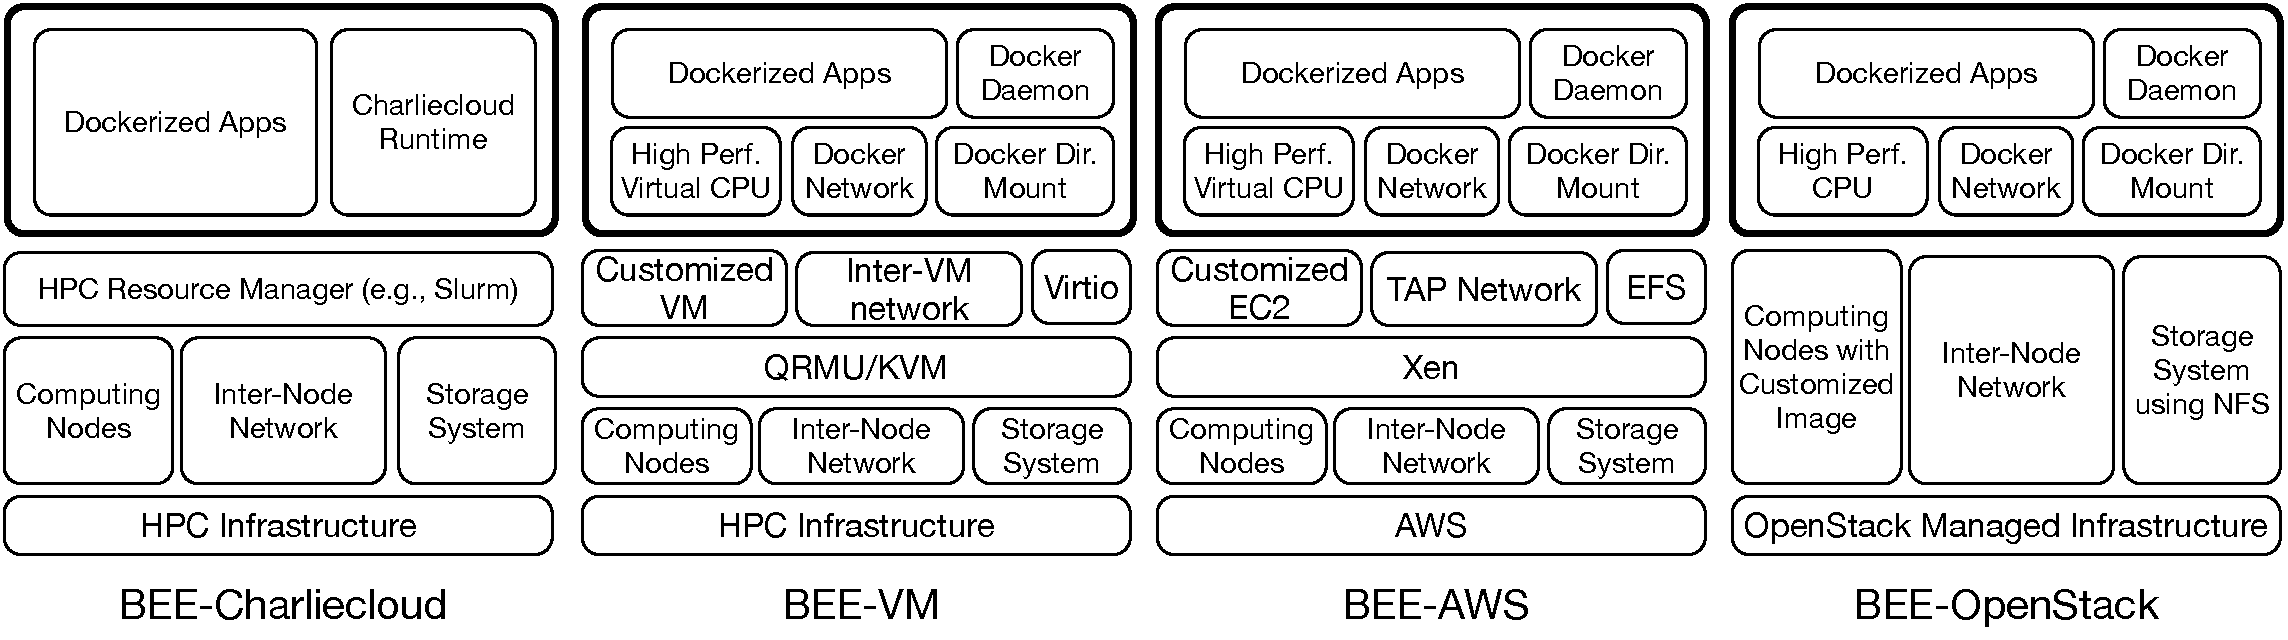
\includegraphics[width=0.8\textwidth]{figures/bee-framework-detail.pdf}
    \caption{BEE Backends}
    \label{bee-backend}
%\vspace*{-1em}
\end{figure*}


\section{BEE design overview}
\label{bee-framework-section}
The goal of \texttt{BEE} is to enable unified experience for users when launching HPC applications across different platforms. This is manifested in two ways: (1) An unified user interface that only requires minimum configuration to launch applications on a platform or switch between different platforms; (2) Similar execution environments for applications on different platforms that aim to enable consistance applcaition execution behavior.

\subsection{User interface}

\lstset{numbers=left,
xleftmargin=1.5em,
frame=single,
framexleftmargin=2em}


\lstset{language=Java}
\begin{lstlisting}[float, escapechar=!,
				   caption= Template of \texttt{beefile}]
 "task_conf": {
  "task_name": <task name>,
  "exec_target": bee_cc|bee_vm|bee_aws|bee_os,
  "general_run": [
  	{ "script": <script 1> },
   { "script": <script 2> }, ...
  ],
  "mpi_run": [
  	{ "script": <script 1> },
   { "script": <script 2> }, ...
  ]
 },
 "docker_conf": {
  "docker_img_tag": <docker image>,
  "docker_username": <username>,
  "docker_shared_dir": <dir>
 },
 "exec_env_conf": {
  "bee_cc": {...} or
  "bee_vm": {...} or
  "bee_aws": {...} or
  "bee_os": {...} 
 }       

\end{lstlisting}

The unified user interface consist of three inputs when launching an application using \texttt{BEE}:
\begin{enumerate}
\item A Docker image containing the application;
\item Run scripts;
\item Task description file -- \texttt{beefile};

\end{enumerate}
The first input is the Docker image containing the application. Then, to run the application when it is deployed on a platform, users need to provide run scrips. Depending on the application, the scripts can be in many forms e.g., Shell scripts, Python scrips, etc. Both the Docker image and run scrips do not need to be modified when switching between different execution platforms. Finally, to hide most complications and still provide enough capability of customization, we propose to use a simple JSON-format task description file (\texttt{beefile}) to handle all the communications between users and \texttt{BEE}. \textbf{Listing 1} shows the template of \texttt{beefile}. Users need to select the suitable execution platform (line 4), provide general sequential run scripts (line 5 - 9) and MPI parallel run scripts (line 10 - 14), information about Dockerized  application (line 16 - 20), and finally provide necessary platform-specific information (line 21 - 26) e.g., node list, credential information. Note different Docker containers, by default, do not share a filesystem at runtime, but many HPC application processes running on different nodes need to have a shared directory to share data, so \texttt{BEE} needs users to specify a directory inside the container (line 16) that will be mounted to a shared host filesystem at runtime. When swithing between platforms, users only need to make modification to the \texttt{beefile}.

\subsection{Execution environment}
To similar execution environments for applications on different platforms that can leads to consistance applcaition execution behavior, \texttt{BEE} backend is proposed. A \texttt{BEE} backend is a component in the \texttt{BEE} framework that can automically build up an HPC-friendly execution environment on a specific class of platforms. We design different \texttt{BEE} backends for different classes of platforms that can all build up the similar execution environment. As for now, \texttt{BEE} has four backends: \texttt{BEE-Charliecloud}, \texttt{BEE-VM}, \texttt{BEE-AWS}, and \texttt{BEE-OpenStack}. These backends are built aiming at four different classes of platforms: texttt{BEE-Charliecloud} supports current and later HPC systems that have Linux user namespace support; \texttt{BEE-VM} supports older HPC systems; \texttt{BEE-AWS} support AWS cloud platform; \texttt{BEE-OpenStack} support OpenStack-based HPC or cloud platforms.

\textbf{Fig. \ref{bee-backend}} shows the hardware and software stack of the fours backend in \texttt{BEE}. The bold rectangle on the top row of each backend indicates the execution environment that each backend provides. Below that are different technologies that are used to enable consistant execution environment. Further below are the three components that are most critical to HPC applications: \textit{computing}, \textit{network}, and \textit{storage}. Each backend is designed to provide similar computing, network, and storage environment for the runtime environment that runs Dockerized HPC applications. This makes sure that applications do not need to be modified to run on another backend and preserving the same execution behavior. We will discuss the design details of each backend in the following sections.

\subsection{Components in \texttt{BEE} framework}
Finally, we introduce other components in \texttt{BEE} framework that help connect the user interface with the backends. \textbf{Fig. \ref{bee-framework}} shows the framework of \texttt{BEE}. The \texttt{BEE Launcher} is the frontend \texttt{BEE} for users to launch a task on \texttt{BEE}-supported platforms, which takes the three inputs mentioned earlier. The core part of \texttt{BEE} is the \texttt{BEE Orchestration Controller}, which is responsible for connecting \texttt{BEE}'s frontend and the fours backends. It takes the task launching requests from \texttt{BEE Launcher} and initiates task launching process through the four backends of \texttt{BEE}. \texttt{BEE Orchestration Controller} uses different threads to manage different tasks at the same time. It also keeps track of the status of each launching process.








